\documentclass{article}
\usepackage[utf8]{inputenc}
\usepackage{amsmath}
\usepackage{amsfonts, amssymb, hyperref,graphicx}
\usepackage[letterpaper, total={7.5in, 9in}]{geometry}
\title{Intermediate Analysis}
\author{Grant Smith }
\date{Spring 2022}

\begin{document}

\maketitle

\section{Sequence Convergence}

\begin{enumerate}
    \item Prove the convergence of $$\lim_{n\rightarrow \infty} (\sqrt{n^{2}+n}-n)$$
    \begin{enumerate}
        \item First, notice that this equation approaches 0.5 as n increases.  Thus, we will be proving:
        $$\forall \epsilon > 0,  \exists N s.t. \forall n > N, \left| \sqrt{n^{2}+n}-n - \frac{1}{2}\right| < \epsilon$$
        \item which is the same as proving both of the following:
        $$ \sqrt{n^{2}+n}-n - \frac{1}{2} < \epsilon$$
        $$ \sqrt{n^{2}+n}-n - \frac{1}{2} > -\epsilon$$
        \item then add $n + 1/2$ to both sides
        $$ \sqrt{n^{2}+n} < \epsilon + n + \frac{1}{2}$$
        $$ \sqrt{n^{2}+n} > -\epsilon + n + \frac{1}{2}$$
        \item square both sides to get:
        $$ n^{2}+n < \epsilon^2 + 2\epsilon n + 2 \epsilon .5 + n^2 + 2 n .5 + .25$$
        $$ n^{2}+n > \epsilon^2 - 2\epsilon n - 2 \epsilon .5 + n^2 + 2 n .5 + .25 $$
        \item cancel the $n^{2}+n$ from both sides to get
        $$ 0 < \epsilon^2 + 2\epsilon n + 2 \epsilon .5 + 0 .25$$
        $$ 0 > \epsilon^2 - 2\epsilon n - 2 \epsilon .5 + 0 .25 $$
        \item Bring the $2\epsilon n$ to the other side
        $$ -2\epsilon n < \epsilon^2  + 2 \epsilon .5 + 0 .25$$
        $$ 2 \epsilon n > \epsilon^2  - 2 \epsilon .5 + 0 .25 $$   
        \item divide by $2\epsilon$ on the second, and divide by $-2\epsilon$ on the first, which flips the direction of the $<$ to $>$.
        $$ n > \frac{\epsilon^2  + 2 \epsilon .5 + 0 .25}{-2\epsilon} $$
        $$ n > \frac {\epsilon^2  - 2 \epsilon .5 + 0 .25}{2 \epsilon} $$
        \item Given that both of these need to be true, and the second is bigger than the first because the second is positive and the first is negative, we can just use the second requirement. Also, notice that this is a decreasing function in $\epsilon$, as desired.
    \end{enumerate}
    \newpage
    \item Prove the convergence of $$\lim_{n\rightarrow \infty} \left(1+\frac{1}{n}\right)^{3}$$
    \begin{enumerate}
        \item First, note that this sequence approaches 1. Thus, we need to prove that:
            $$\forall \epsilon > 0,  \exists N s.t. \forall n > N, \left| \left(1+\frac{1}{n}\right)^{3} - 1\right| < \epsilon$$
        \item Noting that 
        $$\left(1+\frac{1}{n}\right)^{3} > 1$$
        We can drop the absolute value and get
        $$\left(1+\frac{1}{n}\right)^{3} - 1 < \epsilon$$
        \item Move the 1 to the other side to get:
        $$\left(1+\frac{1}{n}\right)^{3} < 1+ \epsilon$$
        \item Take the cube root of both sides
        $$1+\frac{1}{n} < \left(1+ \epsilon\right) ^{\frac{1}{3}}$$
        \item subtract from to both sides
        $$\frac{1}{n} < \left(1+ \epsilon\right) ^{\frac{1}{3}} -1$$
        \item switch positions of the fractions
        $$\frac{1}{\left(1+ \epsilon\right) ^{\frac{1}{3}} -1} < n$$
        \item Switch sides:
        $$n > \frac{1}{\left(1+ \epsilon\right) ^{\frac{1}{3}} -1}$$
        Which increases as $\epsilon$ decreases
        
    \end{enumerate}
    \newpage
    \item Prove the convergence of: 
    $$\lim_{n\rightarrow \infty} \frac{\sin n}{n^{2}}$$
        \begin{enumerate}
        \item First, note that this sequence approaches 0. Thus, we need to prove that:
            $$\forall \epsilon > 0,  \exists N s.t. \forall n > N, \left|\frac{\sin n}{n^{2}}\right| < \epsilon$$
            \item Noting that $n^2 > 0$, we can rewrite as: 
            $$ \frac{\left|\sin n\right|}{n^{2}} < \epsilon$$
            \item Noting that 
            $$\left|\sin n\right| \leq 1 \rightarrow \frac{\left|\sin n\right|}{n^{2}} \leq \frac{1}{n^2} \leq \frac{1}{n} $$
            \item Which means that if we can prove convergence of $1/n$, then we have proven the convergence of the sequence in question. Thus, we want:
            $$\frac{1}{n} < \epsilon$$
            or
            $$\frac{1}{\epsilon} < n$$
            or
            $$n > \frac{1}{\epsilon}$$

        
    \end{enumerate}
                \newpage
            \item Prove that if $\{b_n\}$ is a sequence of positive terms and $b_n \rightarrow b > 0$, then there is a positive lower bound $m > 0$ such that $b_n \geq m$ for all $n$.
\begin{itemize}
    \item If $b_n \rightarrow b > 0$, then for any $\epsilon$ there exists an $N$ such that for all $n > N$, $|b_n - b| < \epsilon$. In particular, if we let $\epsilon = b/2$, then for all $n > N$, we can ensure that $b_n > b/2$, and since $b > 0$, we know that $b/2 > 0$. 
    \item Next, since there are only a finite number of $b_n$ values before N, we can take the minimum of those values. Call this $m'$.  We know that each term is positive, so $m'$ is positive.
    \item Next, we take the minimum of $b/2$ and $m'$, and we can take half of that value as well, and call it m: $\min  \left\{b/2,m'\right\}/2 = m$. This $m$ is one of infinitely many possible lower bounds.
\end{itemize}
\end{enumerate}



\section{Measure Theory Limit}

I really like single sided epsilon balls, and the related idea of single sided limits.  I especially like the deleted versions in which the point about which we're considering is deleted, but I'll explain more about that soon.  Single sided limits great because on either side of a single domain point, a function can behave totally differently. Which is sort of the whole idea. Every point of the continuum is a hinge point between what's on its left and on its right, and the behavior of the two sides can be completely different. So I think single sided limits/neighborhoods are nice because they allow us to treat these two parts of functions in their own right.

Deleted neighborhoods and limits which exclude the individual point are great because they ignore what happens at the single point. And what's also interesting is that they ignore every other point. For example, if you pick a given point, you can make your delta ball small enough to exclude that point. The only situation in which you can include something would be an infinite set in which the point in question is a limit point of that set. So no finite set or individual point is ever considered in a single-sided, deleted neighborhood. And in fact, no point is ever considered in a deleted neighborhood, regardless if it's left or right. And this applies to every single domain point, so under this thinking, no finite set of points or single point ever matters. 

I also really like the idea of considering properties that hold almost everywhere, and ignoring properties that hold almost nowhere. The notion of almost everywhere is awesome because it ignores the behavior of sets with zero measure. This means that any behaviors that are oddities can be ignored. 

And what's interesting about combining these ideas is that if we consider properties in the "almost everywhere" sense, there is no difference between deleted neighborhoods and non-deleted neighborhoods. The singularity of the neighborhood point is ignored under "almost everywhere".  So this idea of almost everywhere is a souped-up version of the deleted neighborhood.

\subsection{Things that do matter}
Limits that diverge such as $\sin \frac{1}{x}$ at $x=0$ and limits that go to infinity, such as 1/x. 

So what we really want to know is how often one of these two things happen. When does the limit diverge, and when does it go to infinity? And we want to know if these happen at all in a function, and if so, how frequently. 

As a small point, I'd like to include $\infty$ in the domain in the sense that $\displaystyle \lim_{x \to \infty} x = \infty$, which I'd include in this section of problems, and I'd also say that $\displaystyle \lim_{x \to \infty} \sin x$ does not exist.  

\subsection{Definition}

$$\forall I, $$

$$\exists B_{\epsilon} , \mu(B_{\delta} \setminus f^{-1}(B_\epsilon)) = 0$$

\subsection{New Theory}

How often can a function break essential continuity?

Working in the context of real functions:

Let's say a function is essentially continuous at a domain point $c$ iff

$$\exists L, \forall B(L), \exists \delta, B_\delta (c) \subseteq \textrm{Cl}(f^{-1}(B(L)))$$

Which means it breaks essential continuity if: 

$$\forall L, \exists B(L), \forall \delta, B_\delta (c) \nsubseteq  \textrm{Cl}(f^{-1}(B(L)))$$

I'm wondering about the size of this set of discontinuities. I'm pretty sure it can at least be countable. But I'm wondering if it can be uncountable or have Lebesgue Measure $> 0$.

\subsection{New Theory From Discontinuity Classification}

I'm going to define an essential discontinuity as the following:

Pick a ball in the domain, and call it $B$.

There exists a nonzero measure set of codomain points, call the set $R$, each of whose elements, $r$, have a ball around them whose inverse image is within $B$.

Some examples of this are $sin(\frac{1}{x})$ and $\frac{1}{x}$ because in both cases, there are a nonzero measure set of codomain points whose surrounding ball has an inverse image inside a ball around the domain point in question.

I think I also need to look into oscillation. The wikipedia page is \url{https://en.wikipedia.org/wiki/Oscillation_(mathematics)/}

We know from \url{https://en.wikipedia.org/wiki/Classification_of_discontinuities/} that the set $D$ of discontinuities is always $F_\sigma$.  I'm pretty sure this can be bigger than countable.  I'm also pretty sure that it can have measure above zero because later in the article, Lebesgue's Theorem is discussed, which says that a function is reimann integrable iff $D$ has measure zero, which makes me think that $D$ can have nonzero measure in general, but it wouldn't be reimann integrable.  But I am pretty sure this includes discontinuities of the first kind such as removable or jumps.  So what I'm wondering is that: we know a function's set of discontinuities can have nonzero measure, but what about if we only discuss discontinuities of the second kind... can the measure of that set be more than zero?

\subsection{Essential Continuity}

In my theory of almost continuity, we can't include jump discontinuities because that would break our properties such as the essential mean value theorem.

\subsection{well-behavedness}

jump discontinuities are pretty well behaved. The do, though, break almost continuity and therefore break mean value theorem, etc. 

But they aren't essential discontinuities, so I'd still say they're pretty well-behaved.

\subsection{sets and partitions of the reals}

I was wondering if you could partition the reals in such a way that around a given point, you could have a nonzero meausre amount of each partition (the original way I thought about it was just to have two partitions and to determine if on either side of the point, you could have some of both partition).  It turns out the answer is yes, and there are a couple good examples.

One example is $f(x) = \sin(1/x)$ at zero. To partition the set, we could have $A$ be the set of $x$ such that $f(x)>0$ and the other partition, $B$ be the set of $x$ such that $f(x)\leq 0$.  Then no matter how small you draw your ball around zero, you'll have some nonzero amount of both $A$ and $B$.

I also wondered if you could do this with infinite partitions. In particular, countable, uncountable, or measure $>0$.  It turns out that you can do it with countable partitions, but I'm not sure about uncountable or greater.  Here is an example of the countable:

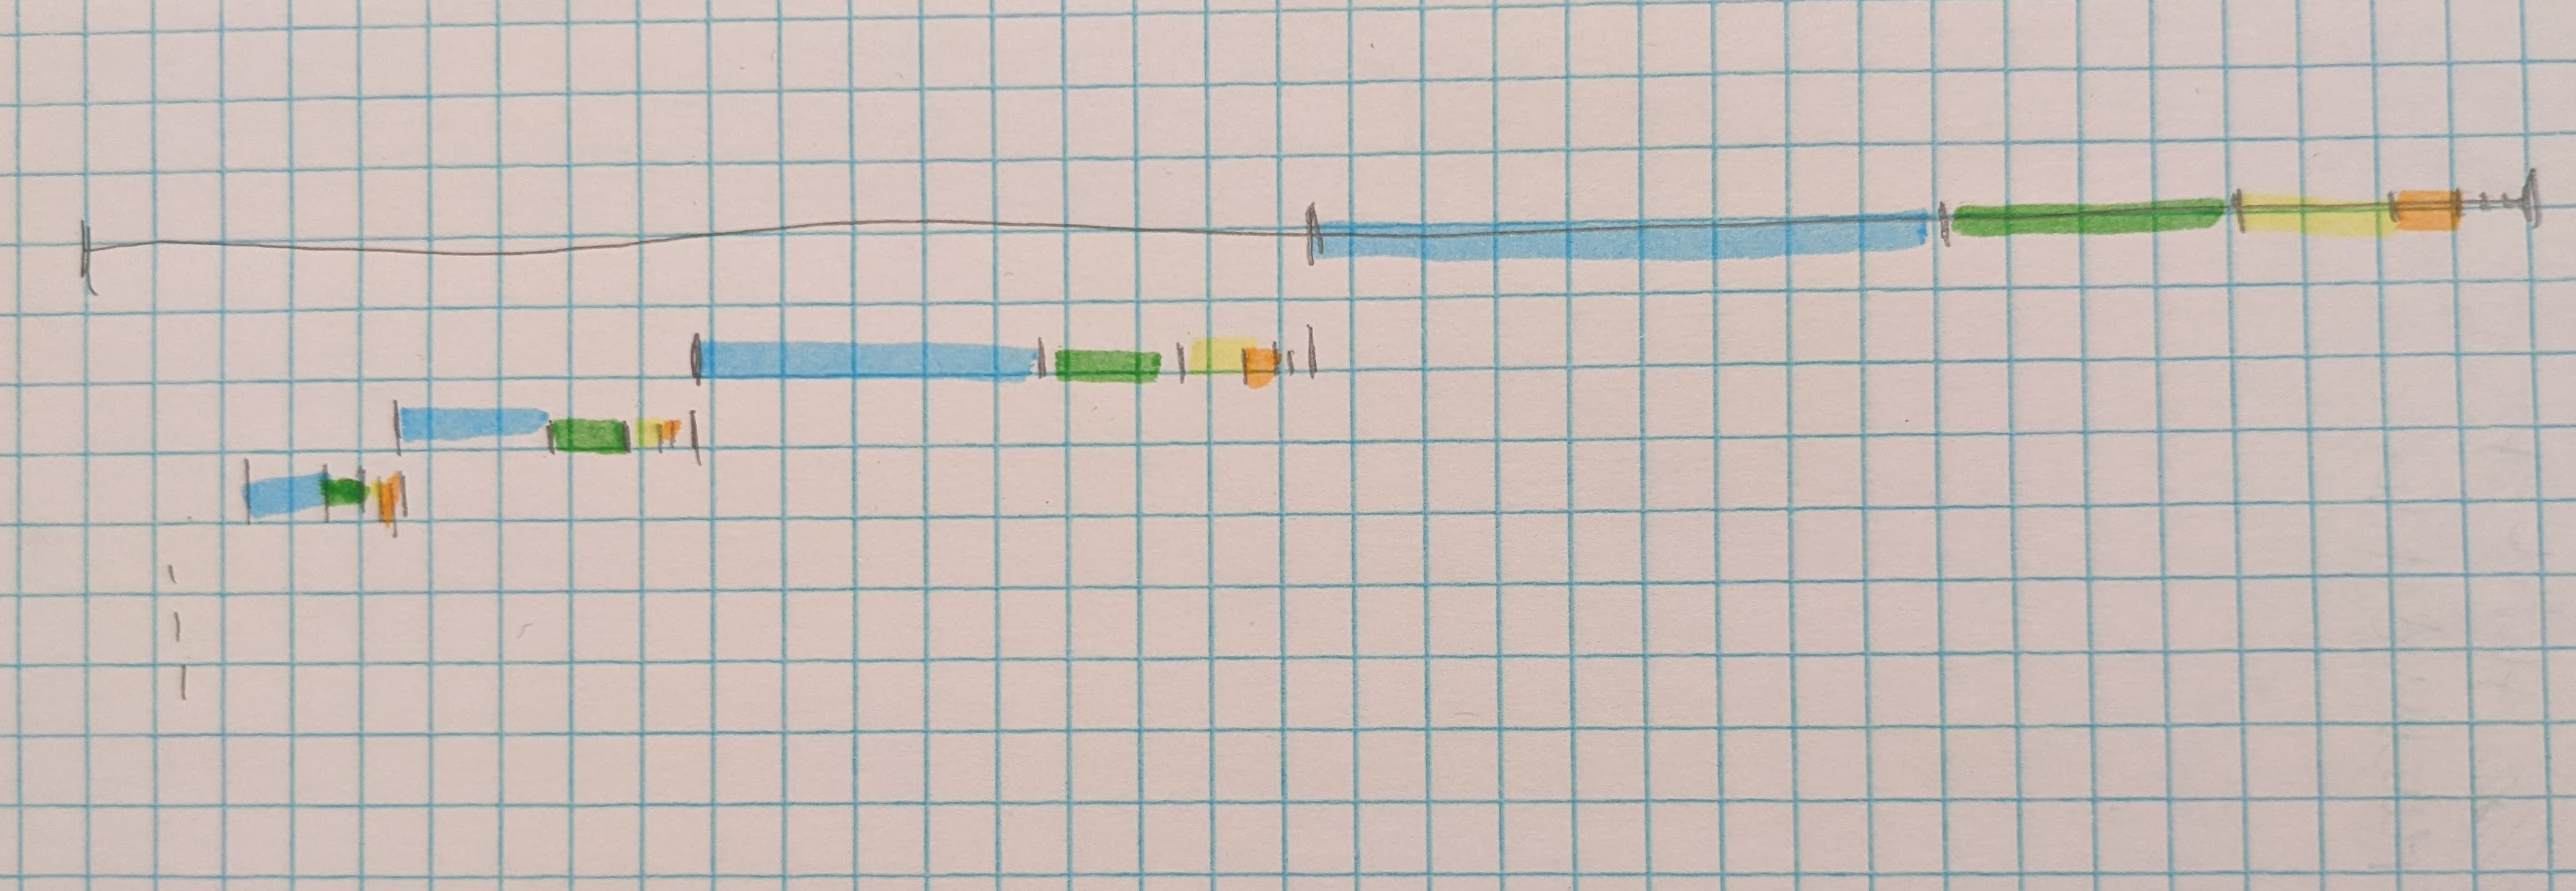
\includegraphics[width=7in]{set-partitions.jpg}
\centering

\end{document}
